%
%
\documentclass[10pt,a4paper]{article}
%\usepackage[latin1]{inputenc}
\usepackage{amsmath}
%\usepackage{amsfonts}
\usepackage{amssymb}
\usepackage{graphicx}
\usepackage{hyperref}
%\usepackage{vmargin}



%%%%%%%%%%%%%%%%%%%%%%%%%%%%%%
\title{The Advanced LIGO Input Mode Cleaner}
\author{Chris Mueller}
%\ligodraft
%%%%%%%%%%%%%%%%%%%%%%%%%%%%%%%%%%%%%%%%%%%%%%%%%%%%%%%%%%%%%%%%%%%%%
\begin{document}

%%%%%%%%%%%%%%%%%%%%%%%%%%%%%%%%%%%%%%%%%%%%%%%%%%%%%%%%%%%%%%%%
\begin{large}
\begin{center}
\begin{LARGE}
\textbf{The Advanced LIGO Input Mode Cleaner}\\
\end{LARGE}
\vspace{0.50in}
\textbf{Chris Mueller} \\
Dept. of Physics, University of Florida\\
\today
\end{center}
\end{large}
\vspace{1pc}
\tableofcontents
\pagebreak[4]

%==================================================================================================
\section{Input Mode Cleaner}

The input mode cleaner is the heart of the input optics, serving simultaneously as a spatial filter, 
polarization filter, frequency reference, and pointing reference.  
It is an in-vacuum, suspended, three mirror cavity with the mirrors hanging from the LIGO small triple 
suspensions \textbf{citation}.  
It has a free spectral range of 9.099 MHz and a finesse of 515.  
The beam is injected along one of the long arms and extracted along the other (see \ref{fig:ioAll}).  
The reflected beam is outfitted with an RF photodiode for Pound-Drever-Hall length sensing \textbf{citation} 
and two wavefront sensors for angular control.  
In addition, a pickoff of the intra-cavity light is extracted behind the curved mirror, MC2, and sent to a 
quadrant photodiode for additional angular information.  

\begin{figure}
	\centering
	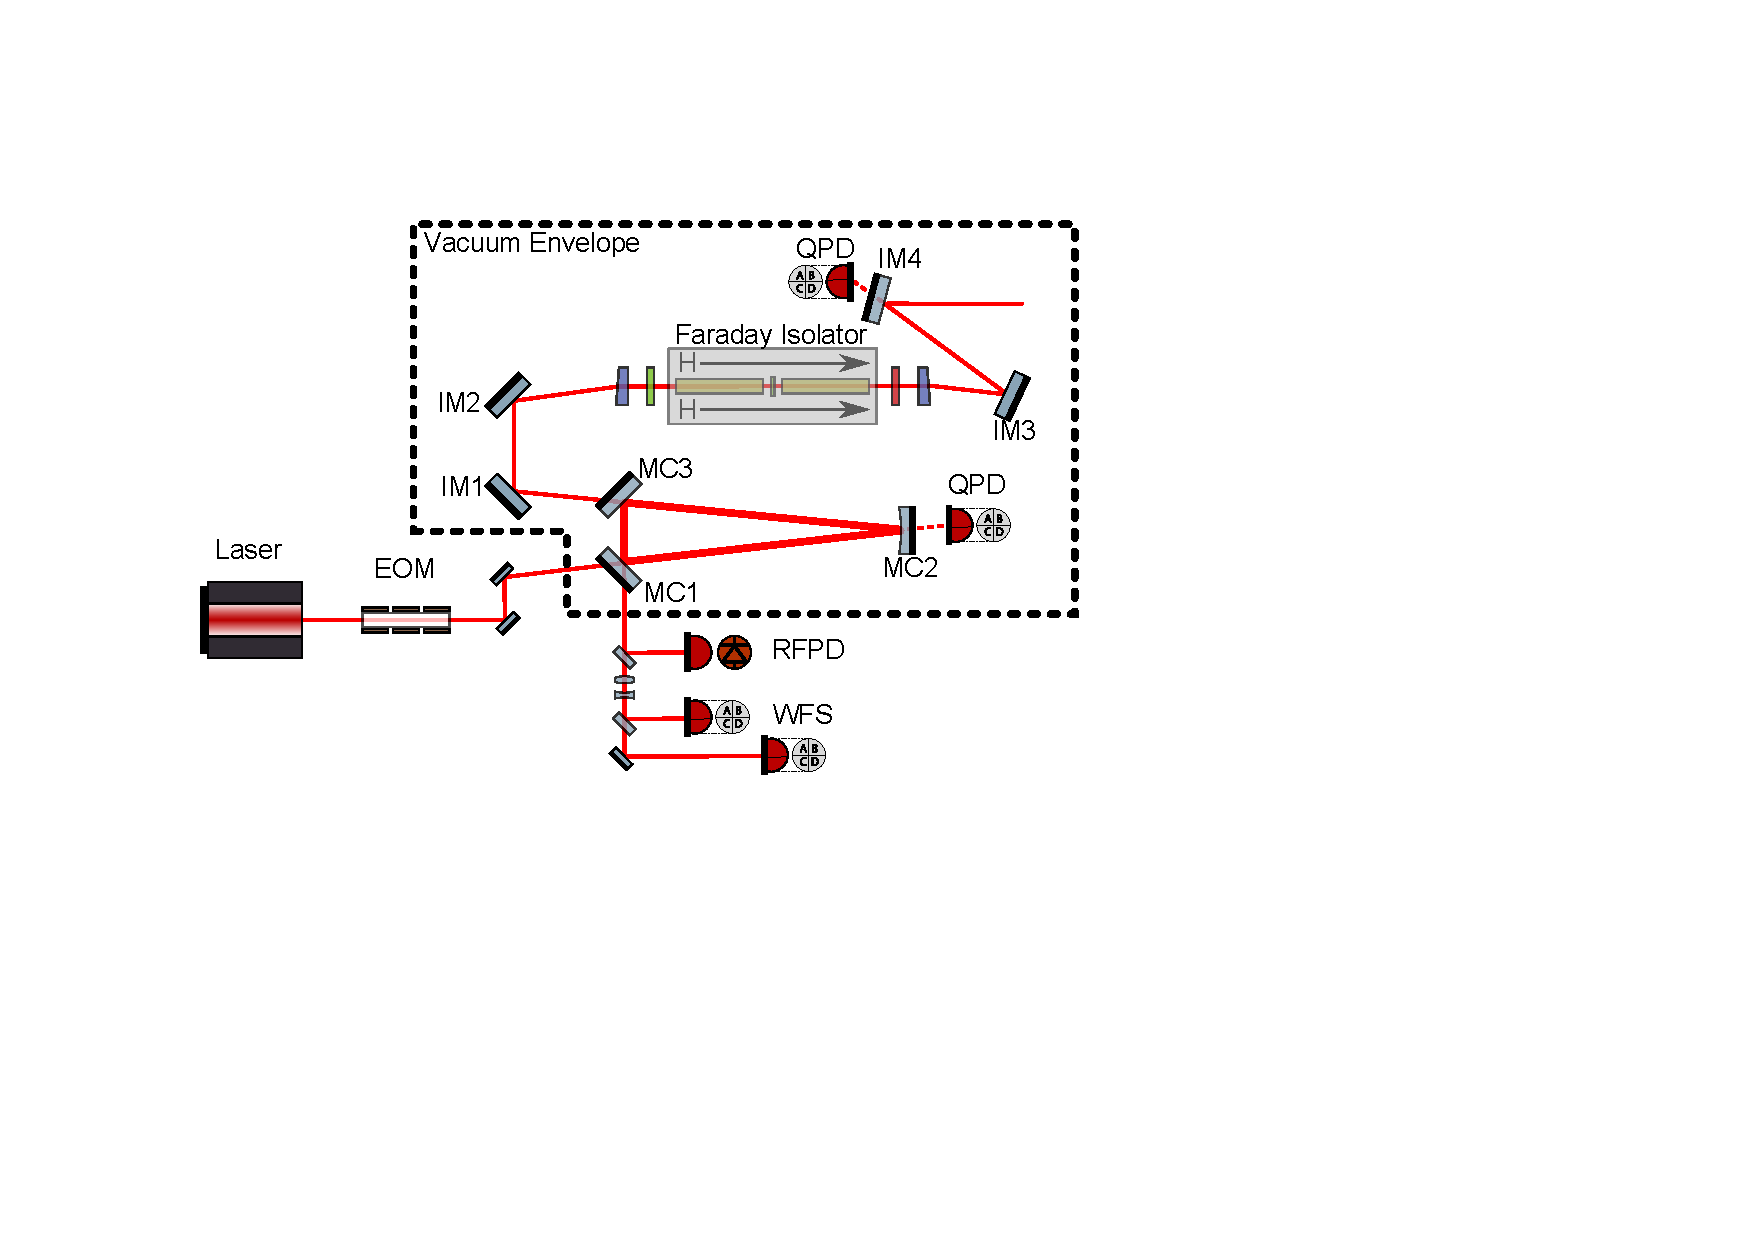
\includegraphics[width=0.9\textwidth, trim=3.5cm 7.5cm 11cm 3.5cm]{IO_Drawing.pdf}
	\caption{A schematic layout of the input optics is shown.  
		The input mode cleaner is represented by the three mirrors MC1, MC2, and MC3.  
		It is an in vacuum triply suspended triangular cavity used as a frequency 
		and pointing reference.  It also passively filters the spatial structure 
		and polarization of the incoming beam.}
	\label{fig:ioAll}
\end{figure}		

%--------------------------------------------------------------------------------------------------
\subsection{Power Budget}

%--------------------------------------------------------------------------------------------------
\subsection{Length Control}
Defining the reflectivity of MC1 and MC3 to be $r$ and assuming the cavity is lossless such that 
$t^2 = 1-r^2$ we can express the complex reflectivity of the cavity as 
\begin{equation}
	r_{IMC} = \frac{r(1+e^{-ik\ell})}{1+r^2e^{-ik\ell}},
\end{equation}
where $k$ is the spatial frequency of the light and $\ell$ is the round trip length of the cavity.  
Notice that this expression is identical to that of a 2 mirror impedance matched cavity except 
for the opposite sign in the denominator due to an odd number of mirrors.  

The most important aspect of this expression for our purposes is that the reflection coefficient 
undergoes a very rapid phase change from $-\pi/2$ on one side of the resonance to $\pi/2$ 
on the other side of the resonance, analogously to mechanical oscillators.  
This phase change can be detected by measuring the beat note between the light passing 
through resonance and a pair of RF sidebands.  
This technique is known as the Pound-Drever-Hall technique\cite{EricBlack}\cite{DreverHall} 
and allows for a very precise comparison between the length of the cavity and the frequency 
of the carrier light.  

As discussed in the requirements section \textbf{reference earlier section} one of the primary 
goals of the input optics is to quiet the laser frequency by at least an order of magnitude 
between 10 Hz and 10 kHz\textbf{reference earlier plot}.  
It is important however that the input optics not impress the length noise of the input mode 
cleaner at low frequencies where the laser frequency is much quieter.  
For this reason 

\begin{figure}
	\centering
	\includegraphics[width=0.8\textwidth,trim = 2.5cm 2cm 2.5cm 1.5cm]{Open_Loop_Tfs.pdf}
	\caption{A model of the open loop transfer functions of the various actuators in the 
		input mode cleaner length/frequency control servo.  
		The triple pendulum suspension of the MC2 mirror is used in a hierarchical scheme to 
		control the length of the cavity at low frequency using the laser frequency as a reference.  
		At higher frequencies the length of the input mode cleaner is more stable and the feedback 
		signal is instead used to stabilize the laser frequency.}
	\label{fig:ControlLoops}
\end{figure}		


%--------------------------------------------------------------------------------------------------
\subsection{Angular Control}

%--------------------------------------------------------------------------------------------------
\subsection{Cavity Pole}
If we define the reflectivity of MC1 and MC3 as $r$ and consider MC2 to be completely reflective, 
then we can express the transmissivity of the IMC as
\begin{equation}
	t_{IMC}=\frac{-t^2e^{-ik(\ell-\ell_3)}}{1+r^2e^{-ik\ell}}.
\end{equation}
Here $t$ is the transmissivity of MC1 and MC3, $\ell$ is the total round trip length, 
$\ell_3$ is the distance from MC1 to MC3, and $k=\tfrac{2\pi f}{c}$ is the spatial frequency 
of the light.  
The cavity is on resonance when $k\ell$ is a equal to $2n\pi+1$ for any $n\in\mathbb{Z}$.  
Notice that transmissivity of the cavity looks identical to that of an impedance matched 
two mirror cavity except for the static phase shift $e^{ik\ell_3}$.  

If we consider the transmissivity of frequencies very near the resonance frequency, 
then we are justified in Taylor expanding the exponential on the bottom to first order 
and the one on the top to 0th order.
Doing so gives an expression which looks like a single pole transfer function;
\begin{equation}
	t_{IMC}\approx e^{ik\ell_3}\frac{\Omega}{\Omega+i\omega},
	\label{eq:PoleApx}
\end{equation}
where
\begin{equation}
	\Omega=\frac{1-r^2}{r^2}\frac{c}{\ell}.
\end{equation}
This parameter, $\Omega$, is commonly referred to as the cavity pole.  
Since the losses in a cavity act to reduce the effective reflectivity of the mirrors, 
a measurement of this parameter is sensitive to the losses in the cavity at the level 
of the errors in the known mirror reflectivities.

There are many ways to measure the cavity pole; 
the simplest way for us was to add a broadband amplitude modulator in between the laser 
and the input mode cleaner.  
To measure the cavity pole we then locked the cavity on the carrier light and added 
an amplitude modulation sideband which we swept from 500 Hz to 100 kHz.  
By demodulating a sample of the light before it entered the cavity and comparing 
it to the demodulated light in transmission of the cavity we were able to 
measure the cavity pole very precisely \ref{fig:cavPole}.  
It should be noted that measuring the cavity pole in this way requires using two 
carefully balanced photodiodes otherwise the measurement will be polluted by the 
relative transfer function of the two photodiodes.

\begin{figure}	
	\centering
	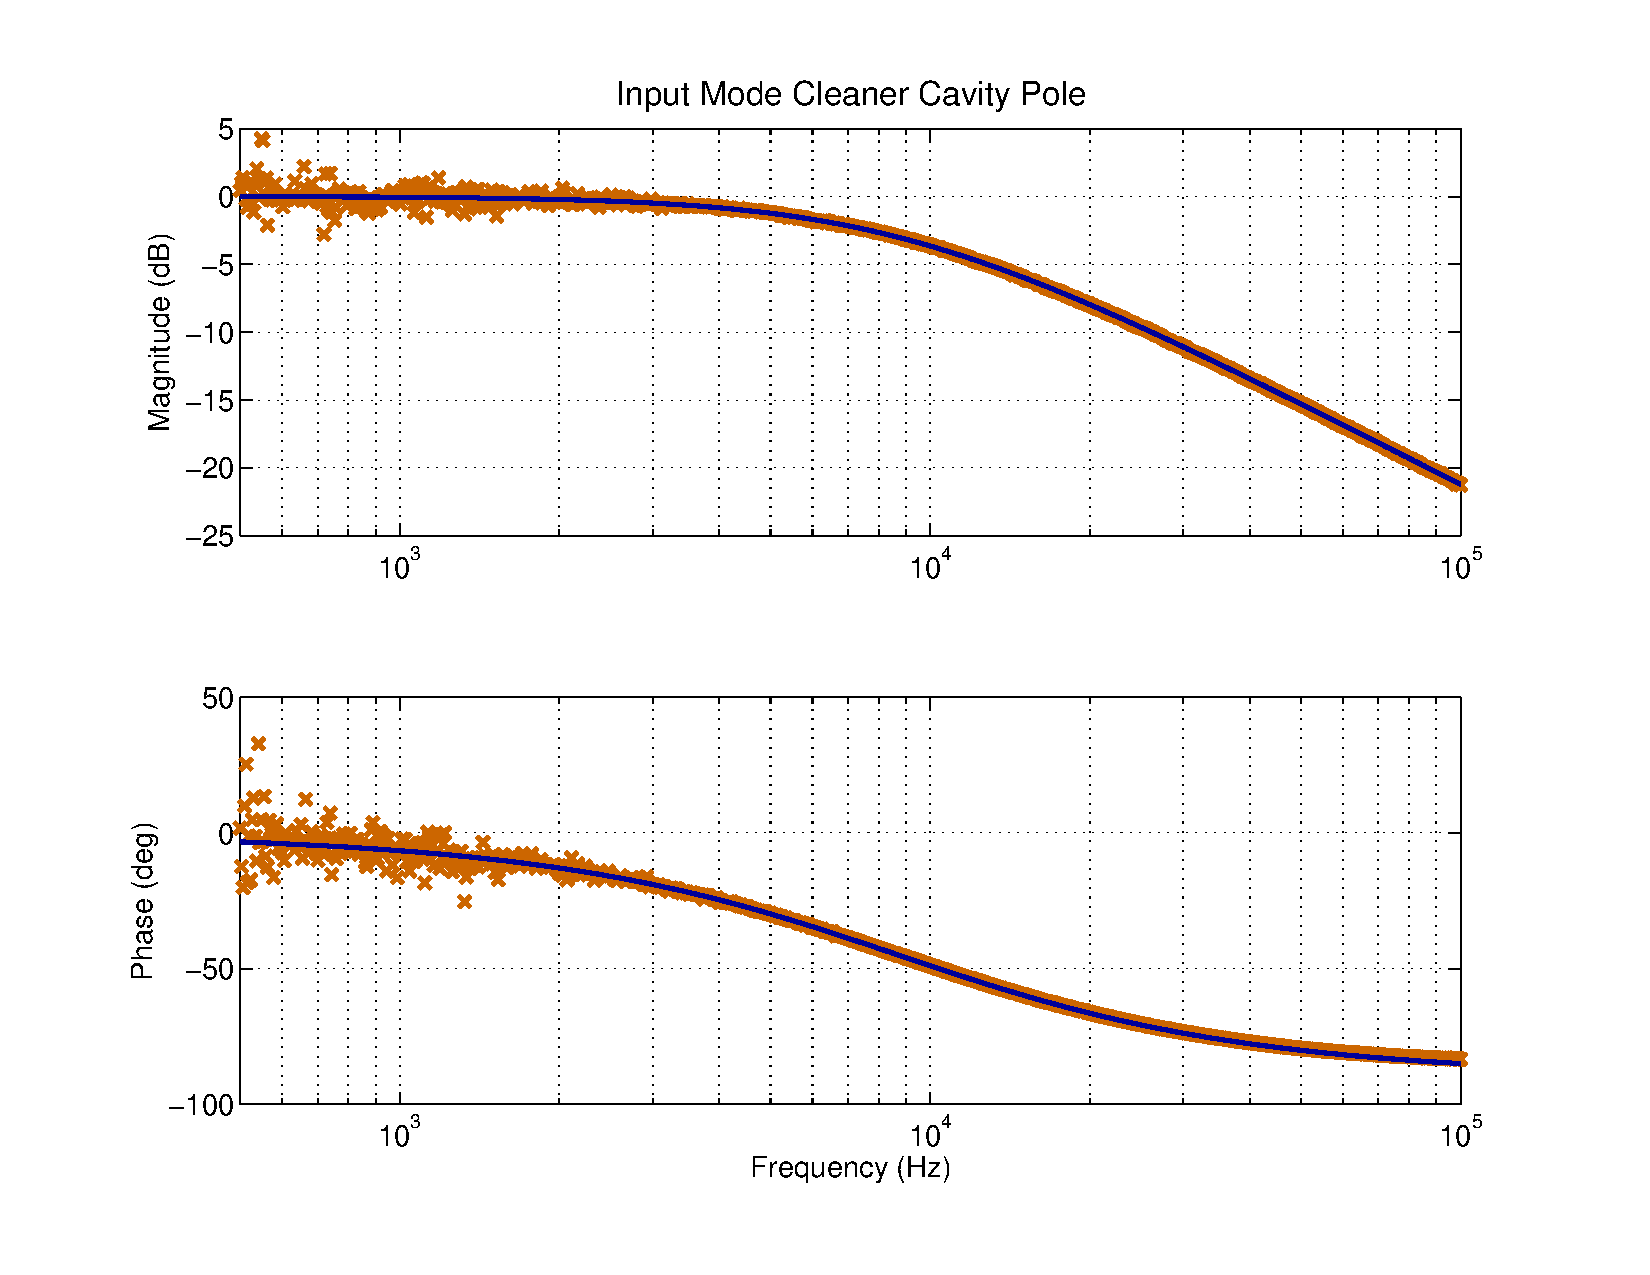
\includegraphics[width = 0.7\textwidth, trim = 2.5cm 1.5cm 2.5cm 1cm]{Cavity_Pole.pdf}
	\caption{The measured IMC cavity pole is shown together with a fit 
		to \eqref{eq:PoleApx}.  The fit has a pole frequency of 8712 Hz 
		which gives a finesse of 522.  These values are within the error 
		bars on the measured mirror reflectivies eliminating the 
		possibility of excessive losses.}
	\label{fig:cavPole}
\end{figure}

The results are shown in figure \ref{fig:cavPole} together with a fit to equation 
\eqref{eq:PoleApx}.  The results give a cavity pole of 8712 Hz which is equivalent 
to a finesse of 522.  
These numbers are exactly what was expected within the error bars of the measured 
reflectivity of the mirrors.  

%--------------------------------------------------------------------------------------------------
\subsection{Noise Budget}

%--------------------------------------------------------------------------------------------------
\subsection{Absorption Measurements}
The absorption in the input mode cleaner can be measured independently of the losses 
by tracking thermally sensitive properties of the mirrors.  
In this case we tracked two different thermally sensitive properties; 
the shift in the local radius of curvature of the optic 
and the shift in the frequency of the fundamental mechanical eigenmode of the mirror.  

The shift in the local radius of curvature of the optic was tracked by 
tracking the higher order mode spacing as a function of power.  
The spacing of the different higher order modes is dependent on the q 
parameter of the cavity which is itself dependent on the local radius of 
curvature of the mirrors.  
The Winkler et. al.\cite{Winkler1991} approximation for the local radius of 
curvature change is
\begin{equation}
	\frac{1}{\delta R}=\delta p=\frac{\alpha}{2\pi\omega^2\kappa}P_a,
\end{equation}
where $\alpha$ is the coefficient of thermal expansion of the mirror,  
$\kappa$ is the thermal conductivity, $\omega$ is the beam size, and
$P_a$ is the power absorbed by the mirror.  
Assuming that the absorption is uniform across the mirrors and the same for 
each mirror ray matrix methods can be used to derive the Gouy phase shift 
of the cavity as a function of power.  
This Gouy phase shift can be expressed equivalently as the shift in the 
frequency location of the 10 peak.  
With these assumptions and approximations the shift in the location of the 10 
peak is given by 
\begin{equation}
	\delta f_{10}=-135.1 \frac{Hz}{ppm\cdot W},
\end{equation}
where the units of ppm is per mirror rather than total.






%--------------------------------------------------------------------------------------------------
\subsection{Thermal Lensing}


\begin{thebibliography}{9}
	\bibitem{drawcite}
		Uses the vector components library developed by Alexander Franzen; available at http://www.gwoptics.org/ComponentLibrary/
	\bibitem{EricBlack}
		Eric Black's PDH paper.
	\bibitem{DreverHall}
		The Drever hall paper on the PDH technique.		
	\bibitem{Winkler1991}
		Winkler, W., K. Danzmann, A. Rudiger, and R. Schilling. Heating by Optical Absorption and 
		the Performance of Interferometric Gravitational-Wave Detectors." Phys. Rev. A 44 117022-7036. 1 December, 1991.
\end{thebibliography}		

\end{document}
